\title{The standard PDE on a manifold}

We state and solve the standard second-order linear PDE on a compact
Riemannian manifold: the potential, diffusion, diffraction and wave
equations.

\newcommand{\R}{\mathbf{R}}
\newcommand{\Z}{\mathbf{Z}}

%\section{0. Overview}
%
%A standard course on partial differential equations should start always with the
%transport equation
%
%$$
%\begin{cases}
%	u_t = u_x &(x,y)\in\R\times\R \\
%	u(x,0) = f(x) &x\in\R
%\end{cases}
%$$
%
%whose solution is~$u(x,t)=f(x-t)$.
%
%This is pretty much a model for any linear first-order PDE with constant
%coefficients.  Then, there are two possible roads: (1) study
%nonlinear first-order PDE, the method of characteristics, hamilton-jacobi,
%hyperbolic systems of conservation laws and so on; (2) study linear
%second-order PDE.  Here we take the second road.
%
%These are the typical cases of linear second order PDE with constant
%coefficients on two variables (ignoring by now any boundary conditions):
%
%\begin{tabular}{ll}
%	$u_t = u_{xx}$         & diffusion, blurring or heat equation \\
%	$u_t = -u_{xx}$        & sharpening, or reverse heat equation \\
%	$u_t = iu_{xx}$        & diffraction or Schrödinger equation \\
%	$u_{tt} = u_{xx}$      & wave equation \\
%	$u_{xx} + u_{yy} = 0$  & Laplace or harmonic equation
%\end{tabular}
%
%The first three cases are particular cases of the form~$u_t=cu_{xx}$ which is
%the~\emph{parabolic} case.  The Laplace equation is the~\emph{elliptic} case
%and the wave equation is the~\emph{hyperbolic} case.
%
%Typically, there is also a non-constant data term that gives some flavour to
%the problem:
%
%\begin{tabular}{ll}
%	$u_t = u_{xx} + f$     & heat equation with a heat source \\
%	$u_{tt} = u_{xx} + f$  & wave equation with an additional force \\
%	$u_{xx} + u_{yy} = f$  & Poisson or potential equation
%\end{tabular}
%
%
%To determine a unique solution, these equations require often boundary
%conditions, for example
%
%$$
%\begin{cases}
%	$u_t = c u_{xx} + f$ & \Omega \\
%
%\end{cases}
%$$


\section{The Laplace-Beltrami spectrum}

Let~$M$ be a compact Riemannian manifold (with or without boundary), and
let~$\Delta$ be its Laplace-Beltrami operator, defined
as~$\Delta=*d*d$, where~$d$ is the exterior derivative (which is independent
of the metric) and~$*$ is the Hodge duality between~$p$-forms
and~$d-p$-forms (which is defined using the metric).

The following are standard results in differential geometry (see e.g.
Warner's book chapter
6~\url{https://link.springer.com/content/pdf/10.1007\%2F978-1-4757-1799-0_6.pdf})

\begin{itemize}
	\item[(1)] There is a sequence of~$\mathcal{C}^\infty(M)$
		functions~$\varphi_n$ and positive
		numbers~$\lambda_n\to\infty$ such that
		$$\Delta\varphi_n=-\lambda_n\varphi_n$$
	\item[(2)] The functions~$\varphi_n$, suitably normalized, are an
		orthonormal basis of~$L^2(M)$.
\end{itemize}

These results generalize Fourier series to an arbitrary smooth manifold~$M$.
Any square-integrable function~$f:M\to\R$ is written uniquely as
$$f(x)=\sum_nf_n\varphi_n(x)$$ and the coefficients~$f_n$ are computed by
$$f_n=\int_Mf\varphi_n.$$  Some particular cases are the habitual Fourier and
sine bases (but not the cosine basis), bessel functions for the disk, and
spherical harmonics for the surface of a sphere.

\begin{tabular}{lccr}
	&$M$ & $\varphi_n$ & $-\lambda_n$ \\
	\hline
	interval & $[0,2\pi]$ & $\sin\left(\frac{nx}{2}\right)$ & $n^2/4$ \\
	circle & $S^1$ & $\sin(n\theta),\cos(n\theta)$ & $n^2$ \\
	square & $[0,2\pi]^2$ &
	$\sin\left(\frac{nx}{2}\right)\sin\left(\frac{m\theta}{2}\right)$ &
	$\frac{n^2+m^2}{4}$ \\
	torus & $(S^1)^2$ & $\sin(nx)\sin(my),\ldots$ & $n^2+m^2$ \\
	disk & $|r|\le1$ & $\sin,\cos(n\theta)J_n(\rho_{m,n}r)$ &
	$\rho_{m,n}$ roots of~$J_n$ \\
	sphere & $S^2$ & $Y^m_l(\theta,\varphi)$ & $l^2+l$
\end{tabular}

The eigenfunctions~$\varphi_n$ are called the vibration modes of~$M$, and the
eigenvalues~$\lambda_n$ are called the (squared) fundamental frequencies of~$M$.

Several geometric properties of~$M$ can be interpreted in terms of the
Laplace-Beltrami spectrum.  For example, if~$M$ has~$k$ connected components,
the first~$k$ eigenfuntions will be supported successively on each connected
component.  On a connected manifold~$M$, the first vibration mode can be
taken to be positive~$\varphi_1\ge0$, thus all the other modes have
non-constant signs (because they are orthogonal to~$\varphi_1$).  In
particular, the sign of~$\varphi_2$ cuts~$M$ in two parts in an optimal way,
it is the Cheeger cut of~$M$, maximizing the perimeter/area ratio of the cut.

The zeros of~$\varphi_n$ are called the nodal curves (or nodal sets) of~$M$,
or also the Chladni patterns.  If~$M$ is a subdomain of the plane, these
patterns can be found by cutting an object in the shape of~$M$, pouring a
layer of sand over it, and letting it vibrate by high-volume sound waves at
different frequencies.  For most frequencies, the sand will not form any
particular pattern, but when the frequency coincides with
a~$\sqrt{\lambda_n}$, the sand will accumulate over the set~$[\varphi_n=0]$,
which is the set of points of the surface that do not move when the surface
vibrates at this frequency.  In the typical case, the number of connected
components of~$[\varphi_n>0]$ grows linearly with~$n$, thus the
functions~$\varphi_n$ become more oscillating (less regular) as~$n$ grows.

Generally, symmetries of~$M$ arise as multiplicities of eigenvalues.
The Laplace-Beltrami spectrum~${\lambda_1,\lambda_2,\lambda_3,\ldots}$ is
closely related, but not identical, to the geodesic length spectrum, that
measures the sequence of lengths of all closed geodesics of~$M$.  The grand
old man of this theory is Yves Colin de Verdière, student of Marcel Berger.

Geometry is not in general a spectral invariant, but non-isometric manifolds
with the same spectrum are difficult to come by.  The first pair of distinct
but isospectral manifolds was wound in 1964 by John Milnor, in dimension 16.
The first example in dimension 2 was found in 1992 by Gordon, Webb and
Wolperd, and it answered negatively the famous question of Marc Kac ``Can you
hear the shape of a drum?'.
In 2018, we have many ways to construct discrete and continuous families of
isospectral manifolds in dimensions two and above.


\section{The standard equations and their explicit solutions}

The classical linear second order equations (potential, heat, wave and
Schrödinger) are all defined in terms of the Laplacian operator in space.
Thus, they can be defined readily on an arbitrary Riemannian manifold~$M$.
If~$M$ is compact, the solution can be found explicitly in terms of the
Laplace-Beltrami eigenfunctions.  Henceforth we will call the expression of a
function~$f:M\to\R$ as~$f=\sum_nf_n\varphi_n$ the Fourier series of~$f$, the
numbers~$f_n$ the Fourier coefficients of~$f$ and so on.

The simplest case is {\bf Poisson equation}
$$
	\Delta u = f
$$
The solution is found by expressing~$u$ and~$f$ as Fourier series and
identifying the coefficients:
$$
u(x) = \sum_n\frac{-f_n}{\lambda_n}\varphi_n(x)
$$
Notice that since~$\lambda_n\to\infty$, the Fourier coefficients of~$u$ tend
to zero faster than those of~$f$, thus~$u$ is more regular than~$f$
(this is obvious from the equation, since~$\Delta u$ is less regular than~$u$).

Another simple case is the {\bf screened Poisson equation}
$$
\Delta u = \alpha u + f
$$
and the solution is found by the same technique:
$$
u(x) = \sum_n\frac{-f_n}{\alpha+\lambda_n}\varphi_n(x)
$$
This is like the regular Poisson equation, but the regularity is enhanced
by~$\alpha$.

The next case is the {\bf heat equation}, also called {\bf diffusion} or {\bf
smoothing} equation:
$$
\begin{cases}
	u_t = \Delta u & (x,t)\in M\times[0,T] \\
	u(x,0)=g(x) & x\in M\\
\end{cases}
$$
This equation requires an initial condition~$g$.  The solution is found by
separation of variables, which leads to a trivial ODE, resulting in
$$
u(x,t)=\sum_ng_ne^{-{\lambda_n}t}\varphi_n(x)
$$
It is immediate to check that this expression is a solution of the heat
equation with initial condition~$g$.  Several properties of the solution are
visible from this form, most notably that~$u(x,\infty)=u_1$ if~$\lambda_1=0$,
or~$1$ otherwise.  A pure vibration mode~$\varphi_n$ decays exponentially to
zero, and the speed of the exponential decay is~$\lambda_n$.

By combining the heat and Poisson equations, we get the {\bf heat equation
with source}:
$$
\begin{cases}
	u_t = \Delta u + f & (x,t)\in M\times[0,T] \\
	u(x,0)=g(x) & x\in M\\
\end{cases}
$$
whose solution is
$$
u(x,t)=\sum_n\left(
\frac{f_n}{\lambda_n}+g_ne^{-{\lambda_n}t}
\right)\varphi_n(x)
$$

The solution of the {\bf reverse heat equation}
$$
\begin{cases}
	u_t = -\Delta u & (x,t)\in M\times[0,T] \\
	u(x,0)=g(x) & x\in M\\
\end{cases}
$$
is formally similar
$$
u(x,t)=\sum_ng_ne^{{\lambda_n}t}\varphi_n(x)
$$
but notice that it blows up, often in a finite time.

Both direct and reverse heat equations are of the form~$u_t=c\Delta u$, whose
solution is~$u(x,t)=\sum_n g_n e^{-c\lambda_n t}\varphi_n(x)$.  The
constant~$c$ is the speed of transmission of heat.  An intermediate behaviour
between~$c>0$ and~$c<0$ happens when~$c=i$.

The {\bf linear Schrödinger equation}, also called {\bf diffraction equation}
$$
\begin{cases}
	w_t = i\Delta w & (x,t)\in M\times[0,T] \\
	w(x,0)=g(x) & x\in M\\
\end{cases}
$$
describes the evolution of a complex-valued function~$w$.  It can be
interpreted as a system of two coupled real equations by writing~$w=u+iv$
(here, assuming a real-valued initial condition~$g$):
$$
\begin{cases}
	u_t = -\Delta v & (x,t)\in M\times[0,T] \\
	v_t = \Delta u & (x,t)\in M\times[0,T] \\
	u(x,0)=g(x) & x\in M\\
	v(x,0)=0 & x\in M\\
\end{cases}
$$
The solution is then
$$
w(x,t)=\sum_n g_n e^{-i\lambda_n t}\varphi_n(x)
$$
or, in terms of~$u$ and~$v$:
$$
\begin{cases}
	u(x,t) = \sum_n g_n\cos\left(\lambda_nt\right)\varphi_n(x) \\
	v(x,t) = \sum_n-g_n\sin\left(\lambda_nt\right)\varphi_n(x) \\
\end{cases}
$$
thus, a pure vibration mode~$\varphi_n$ oscillates periodically, at a
frequency~$\lambda_n$.  In terms of~$|w|$, this phenomenon is called
\emph{diffraction}.

The {\bf wave equation} is
$$
\begin{cases}
	u_{tt} = \Delta u & (x,t)\in M\times[0,T] \\
	u(x,0) = g(x) & x\in M \\
	u_t(x,0) = h(x) & x\in M \\
\end{cases}
$$
notice that it requires an initial condition and an initial speed.  By
linearity, we can deal with these separately, and then sum the
results.  The solution is then
$$
	u(x,t)=\sum_n\left(
	g_n\cos\left(\sqrt{\lambda_n} t\right)
	+
	\frac{h_n}{\sqrt{\lambda_n}}\sin\left(\sqrt{\lambda_n} t\right)
	\right)\varphi_n(x)
$$
Thus, a pure vibration mode~$\varphi_n$ oscillates with
frequency~$\sqrt{\lambda_n}$.

Finally the {\bf wave equation with a force} is the most complex case we treat here:
$$
\begin{cases}
	u_{tt} = \Delta u +f& (x,t)\in M\times[0,T] \\
	u(x,0) = g(x) & x\in M \\
	u_t(x,0) = h(x) & x\in M \\
\end{cases}
$$
The solution
$$
	u(x,t)=\sum_n\left(
	\frac{f_n}{\lambda_n}
	+
	g_n\cos\left(\sqrt{\lambda_n} t\right)
	+
	\frac{h_n}{\sqrt{\lambda_n}}\sin\left(\sqrt{\lambda_n} t\right)
	\right)\varphi_n(x)
$$
is found by the same methods as above.


\section{Discretization and implementation in Octave}

Except in emblematic cases (rectangle, torus, sphere) the eigenfunctions of
an arbitrary manifold~$M$ do not have a closed-form expression.

For practical computations, we are thus restricted to numerical methods in the
discrete case.  The most convenient form for this discretization is to
representd~$M$ as a graph with weights in their edges.  In this context, we
have the following objects
\begin{itemize}
	\item The weighted graph~$G=(V,E)$ where~$V$ is a set of~$n$ vertices.
	\item The Laplacian matrix~$L$ of this graph, which is of
		size~$n\times n$
	\item The space~$\R^n$ is identified with functions~$V\to\R$.
		Thus~$\R^n$ is the discrete version of~$\mathcal{C}^\infty(M)$.
\end{itemize}
typically~$L$ will be a matrix of rank~$n-1$ with a constant eigenvector of
eigenvalue 0.

We can find the eigensystem of~$L$ by calling~\verb+eigs(L)+ in octave, and
transfer the solutions obtained above using the obtained eigenvectors and
eigenvalues.  However, in most cases the solution is more easily obtained by
solving a linear problem.

To fix the ideas we start with a concrete example: a square domain with flat
metric.  The following is a complete program that computes the chladni
figures of a square domain.

\begin{verbatim}
w = 128;                                   # width and height of the domain
p = sparse(1:w-1, 2:w, 1, w, w);           # path graph of length p
A = kron(p, speye(w)) + kron(speye(w), p); # kronecker sum
L = A+A' - diag(sum(A+A'));                # graph laplacian
[f,l] = eigs(L, 64, "sm");                 # eigs of smallest magnitude
\end{verbatim}
%SCRIPT mkdir -p o
%SCRIPT octave <<END
%SCRIPT w = 96;
%SCRIPT p = sparse(1:w-1, 2:w, 1, w, w);
%SCRIPT A = kron(p, speye(w)) + kron(speye(w), p);
%SCRIPT L = A+A' - diag(sum(A+A'));
%SCRIPT [f,l] = eigs(-L'*L, 64, "sm");
%SCRIPT for i=1:64
%SCRIPT         n = sprintf("o/chladni_%03d.png", i);
%SCRIPT         x = reshape(200*double(0<f(:,i)),w,w);
%SCRIPT         iio_write(n, x);
%SCRIPT endfor
%SCRIPT END

After running this code, the ith eigenfunction is \verb+f(:,i)+ and the
eigenvalues are on~\verb+diag(l)+.



\includegraphics{o/chladni_001.png}
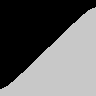
\includegraphics{o/chladni_002.png}
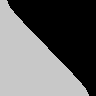
\includegraphics{o/chladni_003.png}
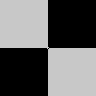
\includegraphics{o/chladni_004.png}
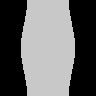
\includegraphics{o/chladni_005.png}
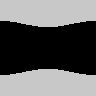
\includegraphics{o/chladni_006.png}
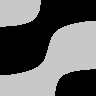
\includegraphics{o/chladni_007.png}
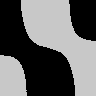
\includegraphics{o/chladni_008.png}

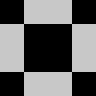
\includegraphics{o/chladni_009.png}
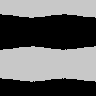
\includegraphics{o/chladni_010.png}
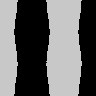
\includegraphics{o/chladni_011.png}
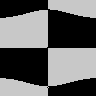
\includegraphics{o/chladni_012.png}
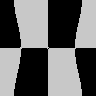
\includegraphics{o/chladni_013.png}
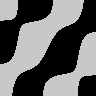
\includegraphics{o/chladni_014.png}
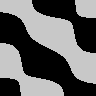
\includegraphics{o/chladni_015.png}
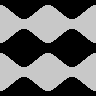
\includegraphics{o/chladni_016.png}

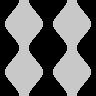
\includegraphics{o/chladni_017.png}
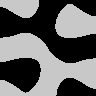
\includegraphics{o/chladni_018.png}
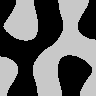
\includegraphics{o/chladni_019.png}
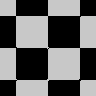
\includegraphics{o/chladni_020.png}

\includegraphics{o/chladni_021.png}
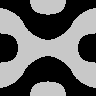
\includegraphics{o/chladni_022.png}
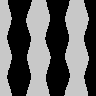
\includegraphics{o/chladni_023.png}
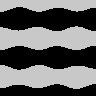
\includegraphics{o/chladni_024.png}

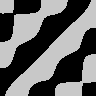
\includegraphics{o/chladni_025.png}
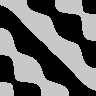
\includegraphics{o/chladni_026.png}
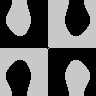
\includegraphics{o/chladni_027.png}
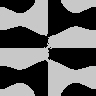
\includegraphics{o/chladni_028.png}

\includegraphics{o/chladni_029.png}
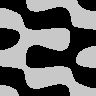
\includegraphics{o/chladni_030.png}
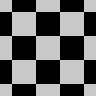
\includegraphics{o/chladni_031.png}
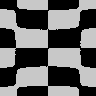
\includegraphics{o/chladni_032.png}

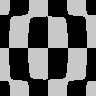
\includegraphics{o/chladni_033.png}
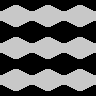
\includegraphics{o/chladni_034.png}
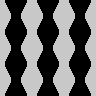
\includegraphics{o/chladni_035.png}
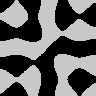
\includegraphics{o/chladni_036.png}
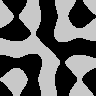
\includegraphics{o/chladni_037.png}
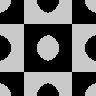
\includegraphics{o/chladni_038.png}
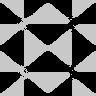
\includegraphics{o/chladni_039.png}
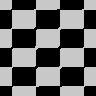
\includegraphics{o/chladni_040.png}

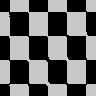
\includegraphics{o/chladni_041.png}
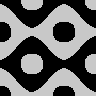
\includegraphics{o/chladni_042.png}

\includegraphics{o/chladni_043.png}
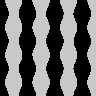
\includegraphics{o/chladni_044.png}
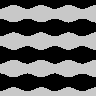
\includegraphics{o/chladni_045.png}
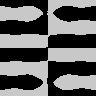
\includegraphics{o/chladni_046.png}
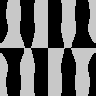
\includegraphics{o/chladni_047.png}
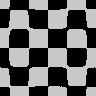
\includegraphics{o/chladni_048.png}


\includegraphics{o/chladni_049.png}
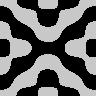
\includegraphics{o/chladni_050.png}
\includegraphics{o/chladni_051.png}
\includegraphics{o/chladni_052.png}
\includegraphics{o/chladni_053.png}
\includegraphics{o/chladni_054.png}
\includegraphics{o/chladni_055.png}
\includegraphics{o/chladni_056.png}

\includegraphics{o/chladni_057.png}
\includegraphics{o/chladni_058.png}
\includegraphics{o/chladni_059.png}
\includegraphics{o/chladni_060.png}
\includegraphics{o/chladni_061.png}
\includegraphics{o/chladni_062.png}
\includegraphics{o/chladni_063.png}
\includegraphics{o/chladni_064.png}



And now, with Dirichlet boundary conditions (slightly different code)

\begin{verbatim}
w = 128;                                    # width and height of the domain
p = sparse(1:w-1, 2:w, 1, w, w) - speye(w); # path graph of length p
A = kron(p, speye(w)) + kron(speye(w), p);  # kronecker sum
L = A + A';                                 # graph laplacian
[f,l] = eigs(L, 64, "sm");                  # eigs of smallest magnitude
\end{verbatim}
%SCRIPT octave <<END
%SCRIPT w = 96;
%SCRIPT p = sparse(1:w-1, 2:w, 1, w, w) - speye(w);
%SCRIPT A = kron(p, speye(w)) + kron(speye(w), p);
%SCRIPT L = A + A';
%SCRIPT [f,l] = eigs(-L'*L, 64, "sm");
%SCRIPT for i=1:64
%SCRIPT         n = sprintf("o/dchladni_%03d.png", i);
%SCRIPT         x = reshape(200*double(0<f(:,i)),w,w);
%SCRIPT         iio_write(n, x);
%SCRIPT endfor
%SCRIPT END


\includegraphics{o/dchladni_001.png}
\includegraphics{o/dchladni_002.png}
\includegraphics{o/dchladni_003.png}
\includegraphics{o/dchladni_004.png}
\includegraphics{o/dchladni_005.png}
\includegraphics{o/dchladni_006.png}
\includegraphics{o/dchladni_007.png}
\includegraphics{o/dchladni_008.png}

\includegraphics{o/dchladni_009.png}
\includegraphics{o/dchladni_010.png}
\includegraphics{o/dchladni_011.png}
\includegraphics{o/dchladni_012.png}
\includegraphics{o/dchladni_013.png}
\includegraphics{o/dchladni_014.png}
\includegraphics{o/dchladni_015.png}
\includegraphics{o/dchladni_016.png}

\includegraphics{o/dchladni_017.png}
\includegraphics{o/dchladni_018.png}
\includegraphics{o/dchladni_019.png}
\includegraphics{o/dchladni_020.png}
\includegraphics{o/dchladni_021.png}
\includegraphics{o/dchladni_022.png}
\includegraphics{o/dchladni_023.png}
\includegraphics{o/dchladni_024.png}

\includegraphics{o/dchladni_025.png}
\includegraphics{o/dchladni_026.png}
\includegraphics{o/dchladni_027.png}
\includegraphics{o/dchladni_028.png}
\includegraphics{o/dchladni_029.png}
\includegraphics{o/dchladni_030.png}
\includegraphics{o/dchladni_031.png}
\includegraphics{o/dchladni_032.png}

\includegraphics{o/dchladni_033.png}
\includegraphics{o/dchladni_034.png}
\includegraphics{o/dchladni_035.png}
\includegraphics{o/dchladni_036.png}
\includegraphics{o/dchladni_037.png}
\includegraphics{o/dchladni_038.png}
\includegraphics{o/dchladni_039.png}
\includegraphics{o/dchladni_040.png}

\includegraphics{o/dchladni_041.png}
\includegraphics{o/dchladni_042.png}
\includegraphics{o/dchladni_043.png}
\includegraphics{o/dchladni_044.png}
\includegraphics{o/dchladni_045.png}
\includegraphics{o/dchladni_046.png}
\includegraphics{o/dchladni_047.png}
\includegraphics{o/dchladni_048.png}

\includegraphics{o/dchladni_049.png}
\includegraphics{o/dchladni_050.png}
\includegraphics{o/dchladni_051.png}
\includegraphics{o/dchladni_052.png}
\includegraphics{o/dchladni_053.png}
\includegraphics{o/dchladni_054.png}
\includegraphics{o/dchladni_055.png}
\includegraphics{o/dchladni_056.png}

\includegraphics{o/dchladni_057.png}
\includegraphics{o/dchladni_058.png}
\includegraphics{o/dchladni_059.png}
\includegraphics{o/dchladni_060.png}
\includegraphics{o/dchladni_061.png}
\includegraphics{o/dchladni_062.png}
\includegraphics{o/dchladni_063.png}
\includegraphics{o/dchladni_064.png}


For completenes, this is the octave code that saves the figures above
\begin{verbatim}
for i=1:64
        n = sprintf("o/chladni_%03d.png", i);
        x = reshape(200*double(0<f(:,i)),w,w);
        iio_write(n, x);
endfor
\end{verbatim}


% vim:set tw=77 filetype=tex spell spelllang=en:
